\documentclass[professionalfonts]{beamer}
\newif\ifita
\itatrue % comment out to hide answers
\itafalse
\usepackage[familydefault,light]{Chivo} 
\usepackage[T1]{fontenc}
\usenavigationsymbolstemplate{}
\usepackage[]{hyperref}
\usepackage{tikz,pgf,pgfarrows,pgfnodes,pgfbaseimage}
\graphicspath{{./Pics/}}
\usetikzlibrary{shapes}
\usepackage{setspace}
\newcommand{\evi}[1]{{\colorbox{yellow!50}{{#1}}}}
\newcommand{\exe}[1]{{\color{black!50}{{#1}}}}
\newcommand{\kw}[1]{{\colorbox{black!30}{\color{white}{#1}}}}
\tikzstyle{nd}=[circle,draw=black,thick,minimum size=.8cm,inner sep=1pt]
\setbeamercovered{transparent}
\usetheme{Singapore}
\tikzstyle{nodo}=[ellipse,draw=black!60,fill=black!10,line width=.7pt,minimum width=.7cm,minimum height=.4cm]
\usecolortheme[named=gray]{structure}
\setbeamercolor{block title}{bg=black!20,fg=black}
\setbeamercolor{block body}{bg=black!10,fg=black}

\usepackage{comment}
%%%%%%%%%%%%%%%%%%%%%
\ifita
\title{Algoritmi Numerici (Parte IV)}
\subtitle{[Lezioni 2 \& 3] Sp-Line (Quadratica e Cubica)}
\else
\title{Numerics (Part IV)}
\subtitle{[Lectures 2 \& 3] Sp-Line Interpolation\\(Quadratic and Cubic)}
\fi
\date{}
\author{Alessandro Antonucci\\{\tt alessandro.antonucci@supsi.ch}}
%%%%%%%%%%%%%%%%%%%%%%%%%%%%
\begin{document}
\maketitle
\setbeamercovered{}
%\setstretch{1.3}
\frame{\frametitle{\ifita Approccio Sp-line \else Sp-line Approach \fi}
\begin{tikzpicture}[rotate=0,domain=-5:10,xscale=.7]
\filldraw [black] (-5,1) circle (1.5pt) node[above] {\tiny $(x_0,y_0)$};
\filldraw [black] (-4,0) circle (1.5pt) node[below] {\tiny $(x_1,y_1)$};
\filldraw [black] (-3,-2) circle (1.5pt) node[below] {\tiny $(x_2,y_2)$};
\filldraw [black] (-2,0) circle (1.5pt);
\filldraw [black] (-1,1) circle (1.5pt);
\filldraw [black] (0,0) circle (1.5pt);
\filldraw [black] (1,1) circle (1.5pt) node[above] {\tiny $(x_{i-1},y_{i-1})$};
\filldraw [black] (2,0) circle (1.5pt) node[below] {\tiny $(x_i,y_i)$};
\filldraw [black] (3,0.04) circle (1.5pt) node[above] {\tiny $(x_{i+1},y_{i+1})$};
\filldraw [black] (4,1) circle (1.5pt);
\filldraw [black] (5,0) circle (1.5pt);
\filldraw [black] (6,-1) circle (1.5pt);
\filldraw [black] (7,0) circle (1.5pt);
\filldraw [black] (8,1) circle (1.5pt);
\filldraw [black] (9,0) circle (1.5pt) node[below] {\tiny $(x_{n-1},y_{n-1})$};
\filldraw [black] (10,-1) circle (1.5pt) node[below] {\tiny $(x_n,y_n)$};
\draw [->] (-5.5,-4) -- (10.5,-4);
\draw [dotted] (-5,1) -- (-5,-4) node[below] {\tiny $x_0$};
\draw [dotted] (-4,0) -- (-4,-4) node[below] {\tiny $x_1$};
\draw [dotted] (-3,-2) -- (-3,-4) node[below] {\tiny $x_2$};
\draw [dotted] (1,1) -- (1,-4) node[below] {\tiny $x_{i-1}$};
\draw [dotted] (2,0) -- (2,-4) node[below] {\tiny $x_i$};
\draw [dotted] (3,0.04) -- (3,-4) node[below] {\tiny $x_{i+1}$};
\draw [dotted] (9,0) -- (9,-4) node[below] {\tiny $x_{n-1}$};
\draw [dotted] (10,-1) -- (10,-4) node[below] {\tiny $x_n$};
{\onslide<2->
\draw[color=red] plot[id=f1,domain=-5:-4] function{1-(x+5)**2};
\draw[color=blue] plot[id=p,domain=-4:-3] function{-2*(x+4)};
\draw[color=green] plot[id=p,domain=-3:-2] function{4*x*x+22*x+28};
\draw[color=magenta] plot[id=p,domain=-2:-1] function{-(x+2)*(5*x+4)};
\draw[color=black] plot[id=p,domain=-1:0] function{3*x*x+2*x};
\draw[color=red] plot[id=p,domain=0:1] function{x-x*(x-1)+.5*x*(x-1)*(x-2)-.125*x*(x-1)*(x-2)*(x-3)};
\draw[color=blue] plot[id=p,domain=1:2] function{x-x*(x-1)+.5*x*(x-1)*(x-2)-.125*x*(x-1)*(x-2)*(x-3)};
\draw[color=green] plot[id=p,domain=2:3] function{x-x*(x-1)+.5*x*(x-1)*(x-2)-.125*x*(x-1)*(x-2)*(x-3)};
\draw[color=magenta] plot[id=p,domain=3:4] function{x-x*(x-1)+.5*x*(x-1)*(x-2)-.125*x*(x-1)*(x-2)*(x-3)};
\draw[color=black] plot[id=p,domain=4:5] function{x-x*(x-1)+.5*x*(x-1)*(x-2)-.125*x*(x-1)*(x-2)*(x-3)};
\draw[color=red] plot[id=p,domain=9:10] function{(.0000*(x-9)**3+.8038*(10-x)**3)/6+(-1)*(x-9)+(0-.8038/6)*(10-x)};
\draw[color=blue] plot[id=p,domain=8:9] function{(.8038*(x-8)**3-3.2153*(9-x)**3)/6+(0-.8038/6)*(x-8)+(1+3.2153/6)*(9-x)};
\draw[color=green] plot[id=p,domain=7:8] function{(-3.2153*(x-7)**3+.0574*(8-x)**3)/6+(1+3.2153/6)*(x-7)+(-.0574/6)*(8-x)};
\draw[color=magenta] plot[id=p,domain=6:7] function{(.0574*(x-6)**3+2.9856*(7-x)**3)/6+(0-.0574/6)*(x-6)+(-1-2.9856/6)*(7-x)};
\draw[color=black] plot[id=p,domain=5:6] function{(2.9856*(x-5)**3+.0*(6-x)**3)/6+(-1-2.9856/6)*(x-5)+(0-0)*(6-x)};}
{\onslide<3->\node[color=red,below] at (-4.2,1.2) {\tiny $f_{0}(x)$};
\node[color=blue,below] at (-3.1,-0.5) {\tiny $f_{1}(x)$};
\node[color=blue,below] at (1.9,1.0) {\tiny $f_{i-1}(x)$};
\node[color=green,below] at (2.9,-.1) {\tiny $f_{i}(x)$};
\node[color=red,below] at (10.1,-0.3) {\tiny $f_{n-1}(x)$};}
\end{tikzpicture}
}


\frame{\frametitle{\ifita Approccio Sp-line \else Sp-line Approach \fi}
\begin{block}{Input}
\begin{itemize}
\ifita
\item Data una serie di $n+1$ punti $\{ (x_i,y_i) \}_{i=0}^n$
\item Tali che $x_{i+1}>x_i$ $\forall i$ \color{gray}{(ordinati da sx a dx)}
\else
\item Given $n+1$ points $\{ (x_i,y_i) \}_{i=0}^n$
\item such that $x_{i+1}>x_i$ $\forall i$ \color{gray}{(sorted from left to right)}
\fi
\end{itemize}
\end{block}
\begin{block}{Output}
\begin{itemize}
\ifita
\item Trovare una funzione $f(x)$ definita tra $x_0$ e $x_{n}$
\item Tale che $f(x_i)=y_i$ {$\forall i=0,1,\ldots,n$ \color{gray}{($f$ passa per i punti)} }
\item $f$ continua {\color{gray}{(opzionalmente anche derivabile $k$ volte)}}
\item Per $x_i \leq x < x_{i+1}$, $f(x)=f_i(x)$ \vskip 2mm (con $f_i$ polinomio di grado fissato)
\else
\item Find a function $f(x)$ defined between $x_0$ and $x_{n}$
\item Such that $f(x_i)=y_i$ {$\forall i=0,1,\ldots,n$ \color{gray}{($f$ crosses the points)}}
\item $f$ continuous {\color{gray}{(optionally first $k$ derivatives)}}
\item For $x_i \leq x < x_{i+1}$, $f(x)=f_i(x)$ \vskip 2mm (with $f_i$ polynomial of given degree)
\fi
\end{itemize}
\end{block}
}

\frame{\frametitle{\ifita Tre (tipi di) Sp-line\else Three (kinds of) Sp-line\fi}
\ifita Congiungo coppie consecutive di punti con: \else Connecting consecutive points by:\fi
\begin{itemize}
\ifita
\item Segmenti di retta (sp-line lineare)
\item Archi di parabola (sp-line quadratica)
\item Archi di cubica (sp-line cubica)
\else
\item Line segments (linear sp-line)
\item Parabolic arcs (quadratic sp-line)
\item Cubic arcs (cubic sp-line)
\fi
\end{itemize}
\vskip 4mm
\begin{itemize}
\ifita
\item Sp-line {\bf lineare}: per due punti passa solo una retta, non ho gradi di libert\`a
(potrei avere punti angolosi)
\item Sp-line {\bf quadratica}: infinite parabole passando per due punti
(impongo derivabilit\`a prima)
\item Sp-line {\bf cubica}: infinite cubiche passando per due punti
(impongo derivabilit\`a prima e seconda)
\else
\item {\bf Linear} sp-line: a single segment for each two points,\\no degrees of freedom
(might have sharp points)
\item {\bf Quadratic} sp-line: infinite parabolic curves crossing two points
(asking continuous derivative)
\item {\bf Cubic} sp-line: infinite cubic curves crossing two points
(asking continuous first and second derivative)
\fi
\end{itemize}
}

\frame{\frametitle{\ifita Bilancio Parametri vs. Vincoli \else Balancing Parameters vs. Constraints \fi}
\begin{itemize} 
\item \ifita Congiungo $n+1$ punti con $n$ segmenti/archi \else Connecting $n+1$ points with $n$ segments/arcs \fi
\item \ifita Sp-line lineare \else Linear sp-line \fi
\begin{itemize}
\ifita
\item due parametri per ogni segmento di retta: $2n$ parametri
\item ogni segmento passa per due punti: $2n$ vincoli
\item $2n-2n=0$ (bilancio in pareggio)
\else
\item two parameters for each line segment: $2n$ parameters
\item each segment connects two points: $2n$ constraints
\item $2n-2n=0$ (balanced)
\fi
\end{itemize}
\item \ifita Sp-line quadratica \else Quadratic sp-line \fi
\begin{itemize}
\ifita
\item ogni arco \`e una parabola (3 parametri): $3n$ parametri
\item ogni parabola passa per due punti: $2n$ vincoli
\item continuit\`a derivata nei punti di raccordo: $n-1$ vincoli
\item $3n-2n-(n-1)=1$ (un parametro libero)
\else
\item every arc is parabolic (3 parameters): $3n$ parameters
\item every arc crosses two points: $2n$ constraints
\item derivative continuous in the junction points: $n-1$ constraints
\item $3n-2n-(n-1)=1$ (a free parameter)
\fi
\end{itemize}
\item \ifita Sp-line cubica \else Cubic sp-line \fi
\begin{itemize}
\ifita
\item ogni arco \`e una cubica (4 parametri) $4n$ parametri
\item ogni cubica passa per due punti: $2n$ vincoli
\item continuit\`a der. I e II nei punti di racc.: $2(n-1)$ vincoli
\item $4n-2n-2(n-1)=2$ (due parametri liberi)
\else
\item every arc is cubic (4 parameters) $4n$ parameters
\item every arc crosses two points: $2n$ constraints
\item der. I and II continuous in the junction points: $2(n-1)$ constraints
\item $4n-2n-2(n-1)=2$ (two free parameters)
\fi
\end{itemize}
\end{itemize}
}

\frame{\frametitle{} \Huge \bf \centering \ifita SP-LINE QUADRATICA \else QUADRATIC SP-LINE\fi}

\frame{\frametitle{\ifita Sp-Line Quadratica \else Quadratic Sp-Line\fi}
\begin{itemize}
\ifita
\item Derivata sp-line quadratica \`e sp-line lineare
\else
\item Derivative of a quadratic sp-line is a linear sp-line
\fi
\ifita
\item Per ogni $i=0,1,\ldots,n$, definisco parametro $z_i:=f'(x_i)$
\else
\item For each $i=0,1,\ldots,n$, let us define $z_i:=f'(x_i)$
\fi
\item \ifita Posso quindi esprimere derivata di \else Rewriting the derivative of \fi $f_i(x_i)$
$$f_i'(x)=\frac{z_{i+1}-z_i}{x_{i+1}-x_i} (x-x_i)+z_i$$
\item \ifita Integro (dalla derivata alla funzione)\else Integrating (from the derivative to the function)\fi
$$f_i(x)=\frac{z_{i+1}-z_i}{x_{i+1}-x_i} \frac{(x-x_i)^2}{2} + z_i (x-x_i) + \alpha_i$$
\item $f_i(x_i)=y_i$ \ifita implica \else implies \fi $\alpha_i=y_i$
\item $f_i(x_{i+1})=y_{i+1}$ \ifita implica invece \else implies \fi
$$y_{i+1}=\frac{z_{i+1}-z_i}{x_{i+1}-x_i} \frac{(x_{i+1}-x_i)^2}{2} + z_i (x_{i+1}-x_i) + y_i$$
\end{itemize}}

\frame{\frametitle{\ifita Sp-line Quadratica (sintesi)\else Quadratic Sp-Line (Recap)\fi}
\Large
\begin{itemize}
\item $z_0$ \ifita dato \else given \fi
\item \ifita ricavo $z_1,z_2,\ldots,z_n$ mediante ricorsione \else recursively getting $z_1,z_2,\ldots,z_n$\fi 
$$z_{i+1} = -z_i + 2 \frac{y_{i+1}-y_i}{x_{i+1}-x_i} $$
\item \ifita uso questi parametri per determinare le parabole: \else these parameters are used to obtain the parabolic curves\fi
$$f_{i}(x) = \frac{z_{i+1}-z_i}{2(x_{i+1}-x_i)}(x-x_i)^2+z_i(x-x_i)+y_i$$ 
\ifita per \else with \fi $x_i \leq x \leq x_{i+1}$
\end{itemize}}

\frame{\frametitle{} \Huge \bf \centering \ifita SP-LINE CUBICA \else CUBIC SP-LINE\fi}
\frame{\frametitle{\ifita Sp-line Cubica \else Cubic Sp-line \fi}
\begin{itemize}
\ifita 
\item Derivata seconda sp-line cubica \`e sp-line lineare
\else
\item Second derivative of a cubic sp-line is a linear sp-line
\fi
\item \ifita Per ogni \else For each \fi $i=0,1,\ldots,n$, \ifita definisco parametro \else let \fi $z_i:=f''(x_i)$
\item \ifita Chiamo \else Let \fi $h_i:=x_{i+1}-x_i$ \ifita distanza punti su asse $x$ \else denote the distance between two points on the $x$-axis \fi
\item \ifita Posso quindi esprimere derivata seconda di \else Rewriting the second derivative of \fi$f_i(x_i)$
$$f_i''(x)=\frac{z_{i+1}}{h_i} (x-x_i)-\frac{z_i}{h_i}(x-x_{i+1})$$
\item \ifita Integro due volte \else Integrating two times \fi
$$f_i'(x)=\frac{z_{i+1}}{2h_i} (x-x_i)^2-\frac{z_i}{2h_i}(x-x_{i+1})^2+\alpha_i$$
$$f_i(x)=\frac{z_{i+1}}{6h_i} (x-x_i)^3-\frac{z_i}{6h_i}(x-x_{i+1})^3+\alpha_i(x-x_i)+\beta_i$$
\end{itemize}}

\frame{\frametitle{\ifita Sp-line Cubica \else Cubic Sp-Line\fi}
$$f_i(x)=\frac{z_{i+1}}{6h_i} (x-x_i)^3-\frac{z_i}{6h_i}(x-x_{i+1})^3+\alpha_i(x-x_i)+\beta_i$$
\ifita Trovo \else Finding \fi $\alpha_i$ \ifita e \else and \fi  $\beta_i$ \ifita imponendo \else by setting \fi $f(x_i)=y_i$ \ifita e \else and \fi $f(x_{i+1})=y_{i+1}$
$$\alpha_i=\frac{y_{i+1}-y_i}{h_i}-\frac{h_i}{6} (z_{i+1}-z_i) \quad \beta_i=y_i-z_i \frac{h_i^2}{6}$$
\ifita Ottengo relazione fra \else Getting relation between \fi $z_{i+1}$, $z_i$, $z_{i-1}$ \ifita con \else where \fi $f_{i-1}'(x_i)=f_i'(x_i)$}

\frame{\frametitle{\ifita Sp-line Cubica (sintesi) \else Cubic Sp-Line (recap)\fi}
\begin{itemize}
\ifita
\item $z_0$ e $z_n$ dati (tipicamente $z_0=0$ e $z_n=0$)
\else
\item $z_0$ and $z_n$ are given (typically $z_0=0$ e $z_n=0$)
\fi

\item \ifita ricavo \else getting \fi $z_1,z_2,\ldots,z_n$ \ifita mediante sistema lineare \else by the linear system \fi
$$h_{i-1} z_{i-1} + 2(h_{i-1}+h_i) z_i + h_i z_{i+1} = 6 \left( \frac{y_{i+1}-y_i}{h_i} - \frac{y_i-y_{i-1}}{h_{i-1}} \right)  $$
$\forall i=1,\ldots,n-1$
\item \ifita uso questi parametri per determinare le cubiche: 
\else with these parameters we write the cubic curves as: \fi
\vskip 1mm
$f_i(x)=$
\footnotesize
$$\frac{z_{i+1}(x-x_i)^3+z_i(x_{i+1}-x)^3}{6h_i} + \left( \frac{y_{i+1}}{h_i} -\frac{h_i}{6} z_{i+1} \right) (x-x_i)
+ \left(  \frac{y_i}{h_{i}} - \frac{h_{i}}{6} z_{i}\right) (x_{i+1}-x)$$
$\forall x_i \leq x \leq x_{i+1}$
\end{itemize}}


\frame{\frametitle{\ifita Sp-line Cubica (sintesi, ii) \else Cubic Sp-Line (recap, ii)\fi}
\begin{itemize}
\item 
\ifita
Se le $x$ dei punti di appoggio sono equidistanti $h_i=h$ per ogni $i$, se poi $h=1$ le formule diventano:
\else
If the $x$ of the points are at the same distance $h_i=h$ for each $i$, and $h=1$, formulae rewrite as:

\fi
\vskip 1mm
$$z_{i-1} + 4 z_i + z_{i+1} = 6 \left( y_{i+1}-2y_i + y_{i-1} \right)$$
\vskip 1mm
$$f_i(x)=\frac{z_{i+1}}{6}(x-x_i)^3+\frac{z_i}{6}(x_{i+1}-x)^3 + $$
$$+\left( y_{i+1} -\frac{z_{i+1}}{6} \right) (x-x_i)
+ \left( y_i - \frac{z_i}{6}\right) (x_{i+1}-x)$$
\end{itemize}}

\end{document}



\frame{\frametitle{} \Huge \bf \centering INTERPOLAZIONE TRIGONOMETRICA}

\frame{\frametitle{Interpolazione trigonometrica}
\begin{itemize}
\item Interpolo $n$ punti di coordinate $\{(x_i,y_i)\}_{i=0}^{n-1}$ ($n$ dispari)
\item Uso la funzione $f(x):= C + \sum_{j=1}^m \left[ a_j \cos (jx) + b_j \sin (jx) \right]$
\item Per bloccare tutti i parametri $n=2m+1$ e quindi $m=\frac{n-1}{2}$
\item Se i punti di appoggio dividono l'intervallo $[0,2\pi]$ in $n$ parti uguali, allora valgono le seguenti formule: 
$$a_j = \frac{2}{n} \sum_{i=0}^{n-1} \left[ y_i \cos(j x_i) \right], \quad \forall j=0,1,\ldots,m$$
$$b_j = \frac{2}{n} \sum_{i=0}^{n-1} \left[ y_i \sin(j x_i) \right], \quad \forall j=1,\ldots,m,$$
e $C=\frac{a_0}{2}$ ($C$ = media aritmetica delle $y$ dei punti di appoggio)
\end{itemize}}

%Se le $x$ dei punti di appoggio sono equidistanti $h_i=h$ per ogni $i$, se poi $h=1$ le formule diventano:
%$$z_{i-1} + 4 z_i + z_{i+1} = 6 \left( y_{i+1}-2y_i + y_{i-1} \right)$$
%$$f_i(x)=z_{i+1}(x-x_i)^3+z_i(x_{i+1}-x)^3 + $$
%$$+\left( y_{i+1} -\frac{z_{i+1}}{6} \right) (x-x_i)
%+ \left( y_i - \frac{z_i}{6}\right) (x_{i+1}-x)$$
%\end{itemize}}

\end{document}

\frame{\frametitle{Un Algoritmo Migliore per Interpolazione Polinomiale}
\begin{itemize}
\item Forma alternativa per polinomio, es. 
$p_3(x)=c_0+c_1 (x-x_0) + c_2(x-x_0)(x-x_1)+c_3(x-x_0)(x-x_1)(x-x_2)$
\item $p_n(x)=\sum_{i=0}^n c_i \left[ \prod_{j=0}^{i-1} (x-x_j) \right] $
\item Impongo passaggio per gli $n+1$ punti:
\vskip 5mm
\begin{center}
$\begin{array}{|ccccc|c|}
\hline
1 & 0 & 0 & \ldots & 0 & y_0\\ 
1 & x_1-x_0 & 0 & \ldots & 0 & y_1\\
&&\ldots&\ldots&&\\
1 & x_n-x_0 & (x_n-x_0)(x_n-x_1) & \ldots & \prod_{j=0}^{n-1} (x_n-x_j)&y_n\\
\hline
\end{array}$
\end{center}
\vskip 3mm
\item Sistema triangolare. Complessit\`a quadratica (e non cubica)!
\end{itemize}}


\frame{\frametitle{Metodo differenze finite}
\begin{itemize}
\item Dati $\{(x_i,y_i)\}_{i=0}^n$
\item Differenze di ordine 1: $f[x_i]:=f(x_i)$ $\forall i=0,\ldots,n$
\item Ordine due $f[x_i,x_{i+1}]:= \frac{f[x_{i+1}]-f[x_i]}{x_{i+1}-x_i}$ $\forall i=0,\ldots,n-1$
\item Ordine tre $f[x_i,x_{i+1},x_{i+2}]:= \frac{f[x_{i+1},x_{i+2}]-f[x_i,x_{i+1}]}{x_{i+2}-x_i}$ $\forall i=0,\ldots,n-2$
\item Ordine quattro $f[x_i,x_{i+1},x_{i+2},x_{i+3}]:= \frac{f[x_{i+1},x_{i+2},x_{i+3}]-f[x_i,x_{i+1},x_{i+2}]}{x_{i+3}-x_i}$ $\forall i=0,\ldots,n-3$
\item Ordine $k$ = Differenza fra ultima e prima ordine $k-1$ \\
diviso ultima $x$ meno prima $x$
\item Ordine $n+1$ $f[x_0,x_1,\ldots,x_n]=\frac{f[x_1,\ldots,x_n]-f[x_0,\ldots,x_{n-1}]}{x_n-x_0}$
\end{itemize}
}

\frame{\frametitle{Metodo differenze finite (ii)}
\begin{itemize}
\item Dispongo valori calcolati su struttura a piramide (es. $n=5$)
\end{itemize}
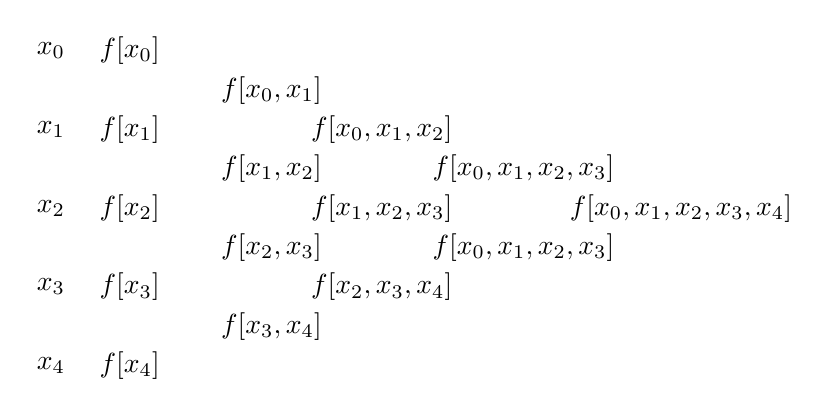
\begin{tikzpicture}
\node[] at (-1,5) {$x_0$};
\node[] at (-1,4) {$x_1$};
\node[] at (-1,3) {$x_2$};
\node[] at (-1,2) {$x_3$};
\node[] at (-1,1) {$x_4$};
\node[] at (0,5) {$f[x_0]$};
\node[] at (0,4) {$f[x_1]$};
\node[] at (0,3) {$f[x_2]$};
\node[] at (0,2) {$f[x_3]$};
\node[] at (0,1) {$f[x_4]$};
\node[] at (1.8,4.5) {$f[x_0,x_1]$};
\node[] at (1.8,3.5) {$f[x_1,x_2]$};
\node[] at (1.8,2.5) {$f[x_2,x_3]$};
\node[] at (1.8,1.5) {$f[x_3,x_4]$};
\node[] at (3.2,4) {$f[x_0,x_1,x_2]$};
\node[] at (3.2,3) {$f[x_1,x_2,x_3]$};
\node[] at (3.2,2) {$f[x_2,x_3,x_4]$};
\node[] at (5,3.5) {$f[x_0,x_1,x_2,x_3]$};
\node[] at (5,2.5) {$f[x_0,x_1,x_2,x_3]$};
\node[] at (7,3) {$f[x_0,x_1,x_2,x_3,x_4]$};
\end{tikzpicture}}

\frame{\frametitle{Complessit\`a spaziale da $O(n^2)$ a $O((n)$}
\begin{itemize}
\item Dispongo valori calcolati su struttura a piramide (es. $n=5$)
\end{itemize}
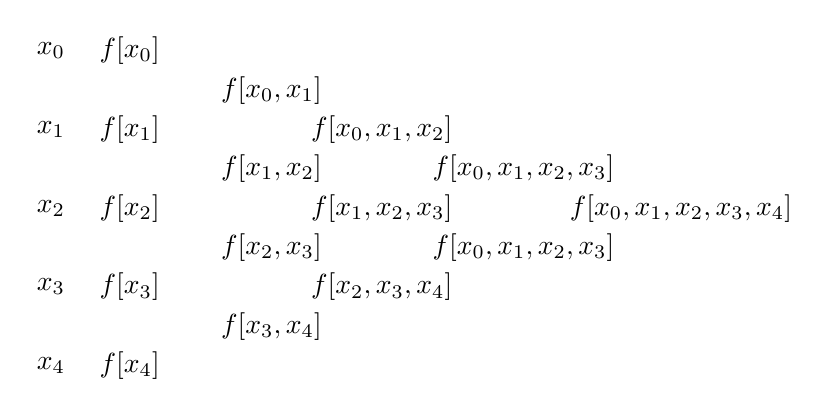
\begin{tikzpicture}
\node[] at (-1,5) {$x_0$};
\node[] at (-1,4) {$x_1$};
\node[] at (-1,3) {$x_2$};
\node[] at (-1,2) {$x_3$};
\node[] at (-1,1) {$x_4$};
\node[] at (0,5) {$f[x_0]$};
\node[] at (0,4) {$f[x_1]$};
\node[] at (0,3) {$f[x_2]$};
\node[] at (0,2) {$f[x_3]$};
\node[] at (0,1) {$f[x_4]$};
\node[] at (1.8,4.5) {$f[x_0,x_1]$};
\node[] at (1.8,3.5) {$f[x_1,x_2]$};
\node[] at (1.8,2.5) {$f[x_2,x_3]$};
\node[] at (1.8,1.5) {$f[x_3,x_4]$};
\node[] at (3.2,4) {$f[x_0,x_1,x_2]$};
\node[] at (3.2,3) {$f[x_1,x_2,x_3]$};
\node[] at (3.2,2) {$f[x_2,x_3,x_4]$};
\node[] at (5,3.5) {$f[x_0,x_1,x_2,x_3]$};
\node[] at (5,2.5) {$f[x_0,x_1,x_2,x_3]$};
\node[] at (7,3) {$f[x_0,x_1,x_2,x_3,x_4]$};
\end{tikzpicture}}
\end{document}

\begin{center}
{\onslide<1->
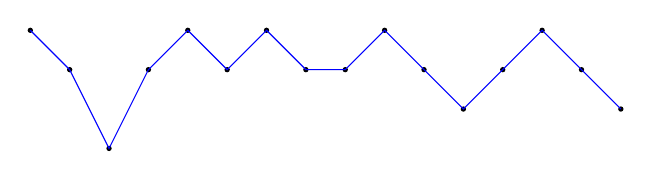
\begin{tikzpicture}[rotate=0,domain=-5:10,scale=.5]
\filldraw [black] (-5,1) circle (1.5pt);
\filldraw [black] (-4,0) circle (1.5pt);
\filldraw [black] (-3,-2) circle (1.5pt);
\filldraw [black] (-2,0) circle (1.5pt);
\filldraw [black] (-1,1) circle (1.5pt);
\filldraw [black] (0,0) circle (1.5pt);
\filldraw [black] (1,1) circle (1.5pt);
\filldraw [black] (2,0) circle (1.5pt);
\filldraw [black] (3,0) circle (1.5pt);
\filldraw [black] (4,1) circle (1.5pt);
\filldraw [black] (5,0) circle (1.5pt);
\filldraw [black] (6,-1) circle (1.5pt);
\filldraw [black] (7,0) circle (1.5pt);
\filldraw [black] (8,1) circle (1.5pt);
\filldraw [black] (9,0) circle (1.5pt);
\filldraw [black] (10,-1) circle (1.5pt);
{\onslide<1->
\draw[color=blue] (-5,1) -- (-4,0) -- (-3,-2) -- (-2,0) -- (-1,1) -- (0,0) -- (1,1) -- (2,0) -- (3,0) -- (4,1) -- (5,0) -- (6,-1) -- (7,0) -- (8,1) -- (9,0) -- (10,-1);}
\end{tikzpicture}}
\end{center}

